\section{Definicja wymagań}
Celem tej części projektu było zaprojektowanie i napisanie oprogramowania robota.
Określono, że będą dwa rodzaje aktorów ludzkich wchodzących w interakcje z systemem:
\begin{itemize}
    \item administrator -- jest tylko jeden i ma dostęp do wszystkich ustawień i zarządzania pozostałymi użytkownikami;
    \item pracownik ochrony -- ma dostęp do kluczowych funkcjonalności;
\end{itemize}
Funkcjonalności, jakie ma posiadać system zostały zdefiniowane na diagramie przypadków użycia \ref{rys:usecases}.
\begin{figure}[H]
    \centering 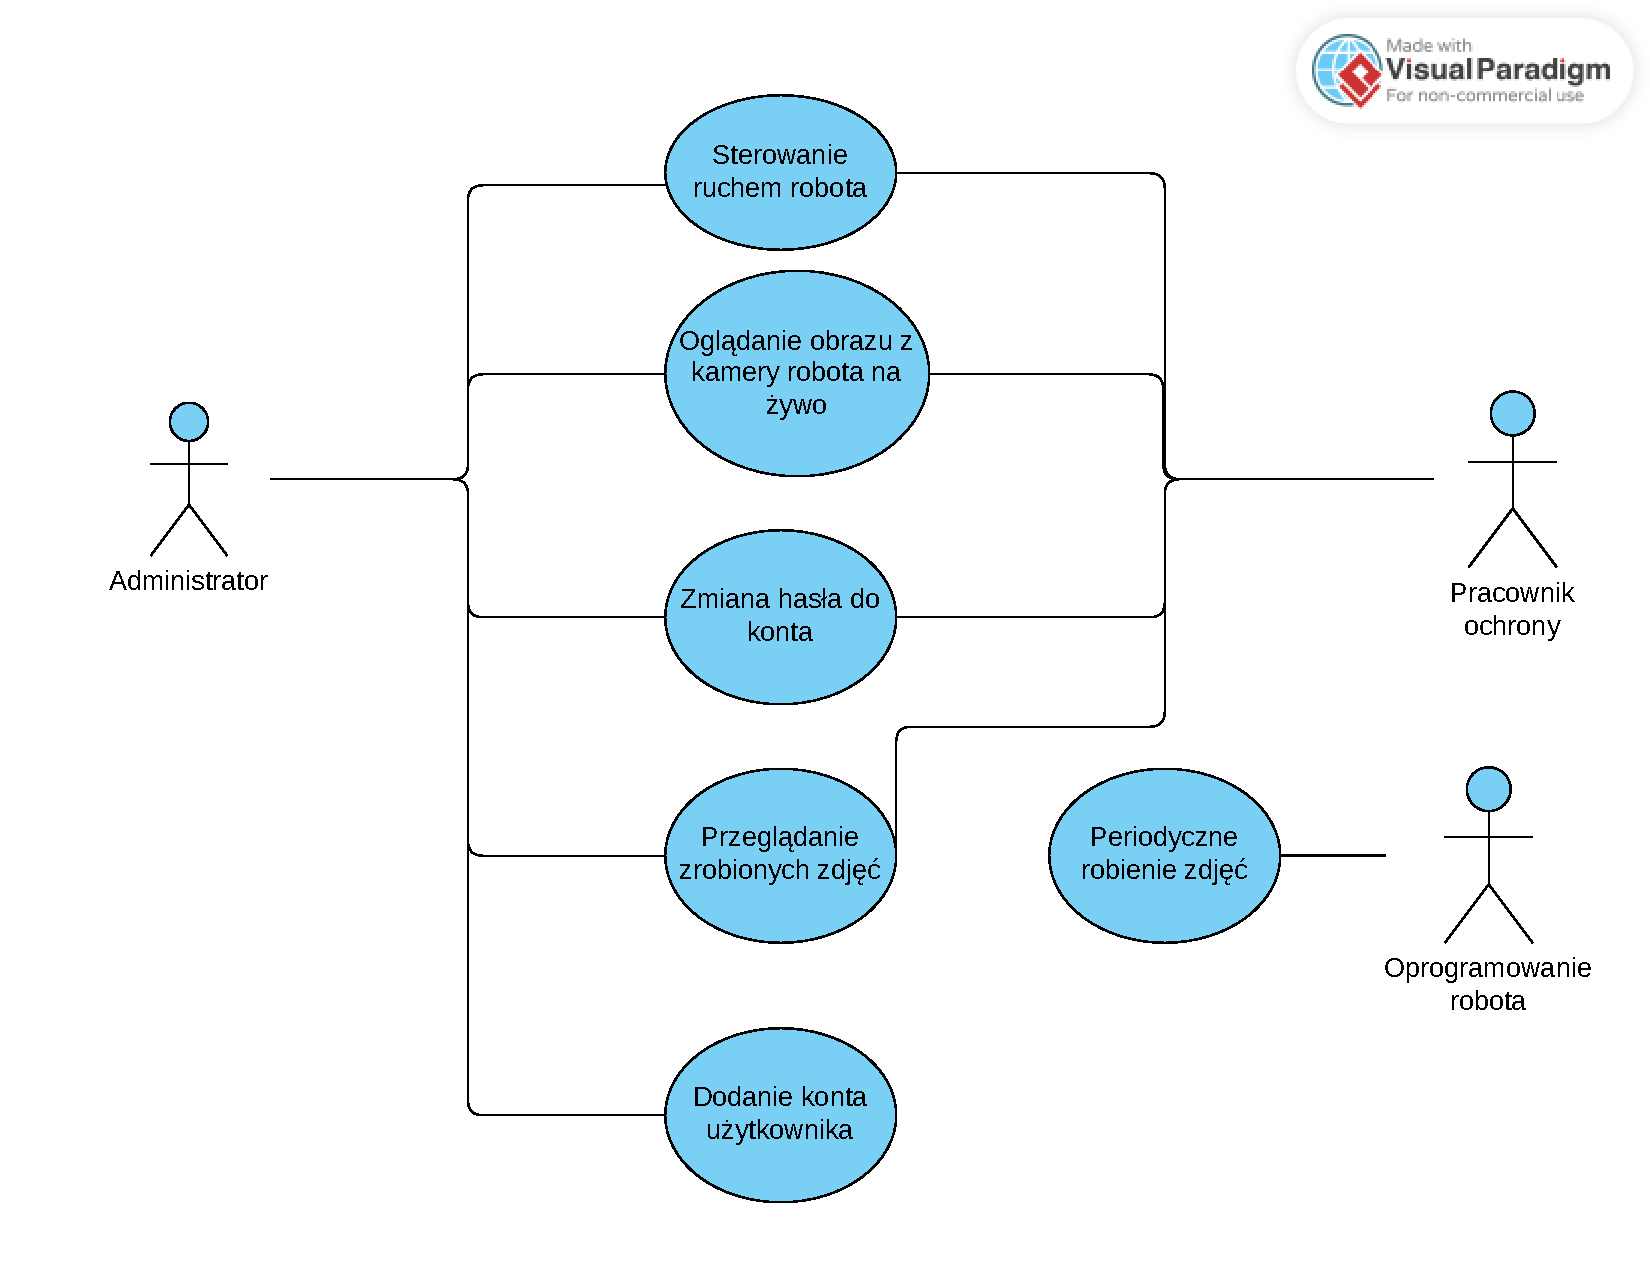
\includegraphics[width=0.8\linewidth]{robot_usecases.pdf}
    \caption{Diagram przypadków użycia}
    \label{rys:usecases}
\end{figure}

\section{Architektura systemu}
Zdecydowano się na interfejs użytkownika w formie aplikacji przeglądarkowej (webowej).
Rozwiązanie to pozwala na dostęp do systemu bez instalacji żadnego oprogramowania.
Ponadto taka forma aplikacji pozwala na dostęp przez szeroką gamę urządzeń końcowych -- komputery, smartfony, tablety itp.

Zgrubny podział aplikacji jest na:
\begin{itemize}
    \item Frontend \\
    Aplikacja uruchamiana w przeglądarce użytkownika.
    Prezentuje dane przychodzące z robota użytkownikowi.
    Przesyła do backendu dane pochodzące od użytkownika.
    \item Backend \\
    Aplikacja działająca na sprzęcie robota.
    Wysyłająca dane do frontendu i przetwarzająca przychodzące dane.
    Steruje zachowaniem robota.
\end{itemize}

Na backendzie ze względu na różnorodną i wielowarstwową funkcjonalność aplikacji zdecydowano się na architekturę mikroserwisową.
Wysokopoziomowa komunikacja modułów między sobą ukazana jest na diagramie komponentów \ref{rys:components}.
\begin{figure}[H]
    \centering 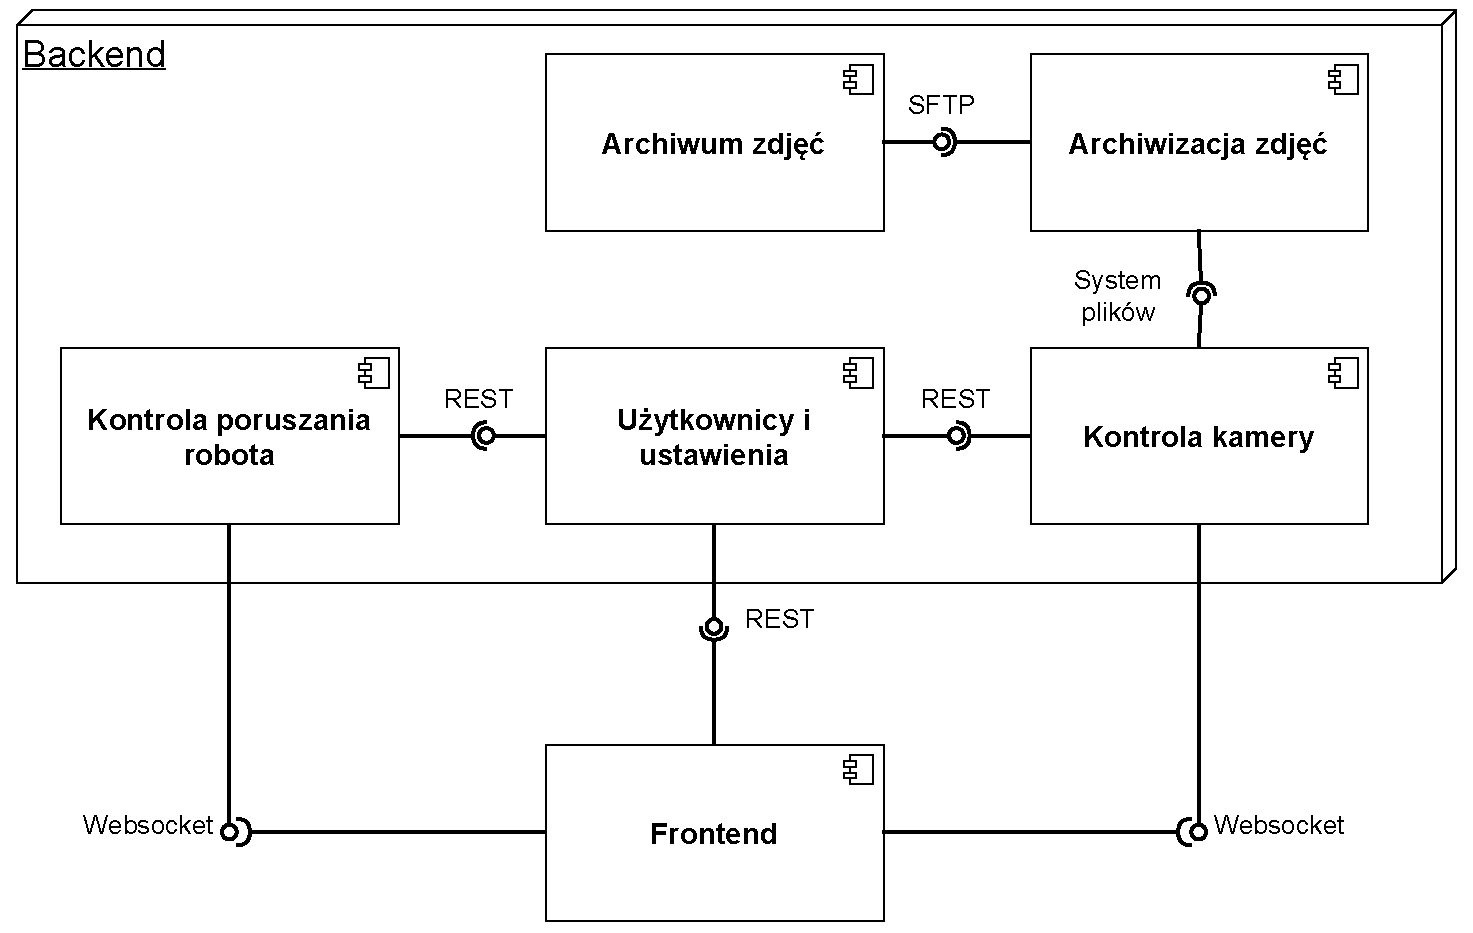
\includegraphics[width=1.0\linewidth]{robot_components.pdf}
    \caption{Diagram komponentów}
    \label{rys:components}
\end{figure}

\section{Wdrożenie}
Wdrożona aplikacja ma działać na sprzęcie samego robota i na urządzeniach końcowych użytkowników.
Wykorzystując możliwości minikomputera Raspberry Pi stawiany jest na nim serwer backendu i frontendu.
Jedynym wykorzystaniem zewnętrznej infrastruktury jest zewnętrzny serwer na pliki, gdzie archiwizowane są zdjęcia.
Architektura wdrożeniowa przedstawiona jest na schemacie \ref{rys:deploy}.

We wdrożeniu wszystkie moduły backendowe są schowane za reverse proxy, które stanowi odpowiednio skonfigurowany serwer HTTP \href{https://nginx.org/}{\textit{nginx}}.
Do uruchamiania całej aplikacji napisany został skrypt w bashu.
Skrypt ten z kolei jest uruchamiany przez specjalnie napisany serwis \textit{systemd}\footnote{\textit{systemd} to menadżer systemu i usług w wielu dystrybucjach systemu operacyjnego GNU/Linux.}.

Jeśli chodzi o architekturę sieciową, to robot jest połączony do internetu przez bezprzewodową sieć Wi-Fi.
Ponadto, administrator może podłączyć maszynę do wirtualnej sieci prywatnej.
\href{https://www.zerotier.com/}{\textit{ZeroTier}} jest popularnym tego typu oprogramowaniem wykorzystanym w tym projekcie.
Dzięki temu rozwiązaniu użytkownicy robota mogą korzystać z systemu robota w jakimkolwiek miejscu z dostępem do internetu.
Jednocześnie \textit{ZeroTier} szyfruje cały ruch sieciowy od końca do końca, co gwarantuje bezpieczeństwo i prywatność.
\begin{figure}[H]
    \centering 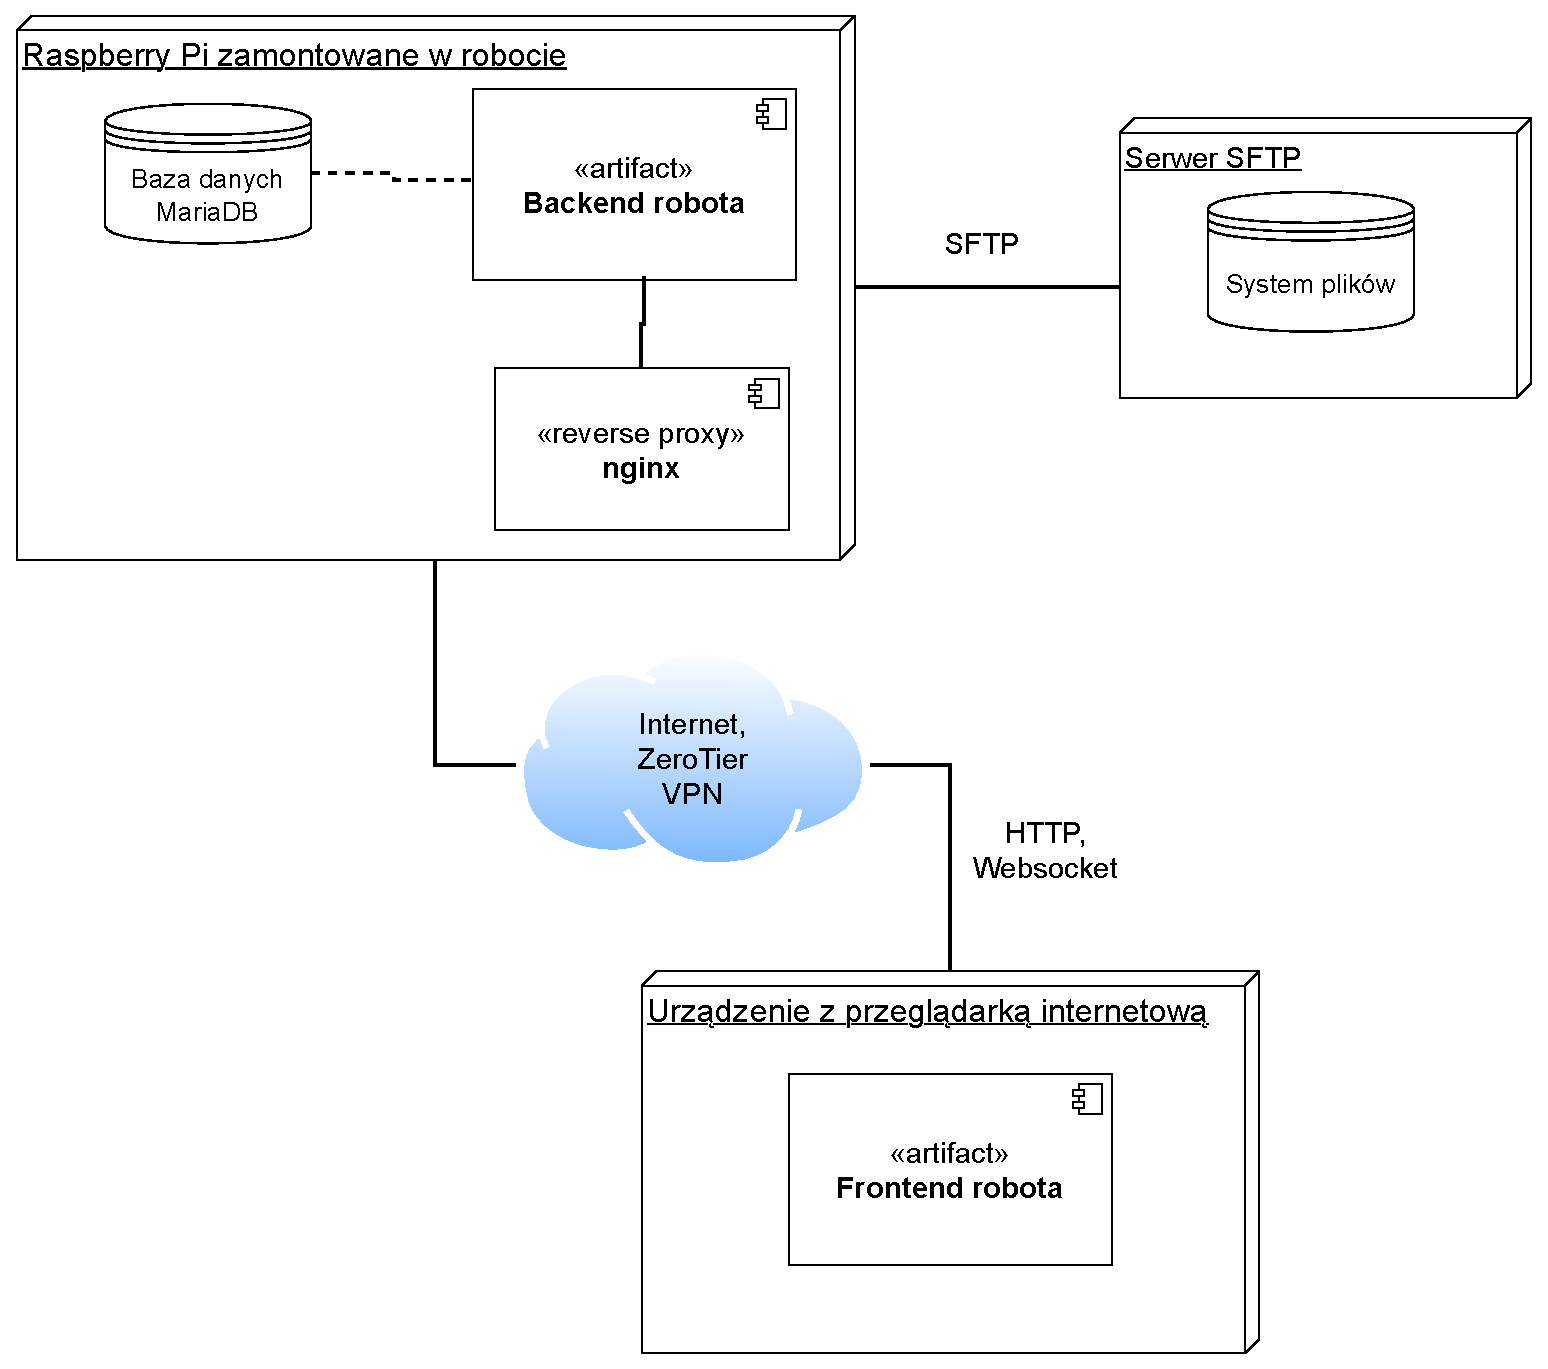
\includegraphics[width=0.9\linewidth]{robot_deploy.pdf}
    \caption{Diagram wdrożenia}
    \label{rys:deploy}
\end{figure}

\section{Serwis użytkowników i ustawień}
\label{main_backend}
Program ten jest serwerem HTTP wystawiającym API typu REST do komunikacji z frontendem.
Przechowuje dane w lokalnej, relacyjnej bazie danych - \textit{MariaDB}.
Aplikacja jest napisana w języku Python i wykorzystuje popularny framework do aplikacji internetowych - \href{https://flask.palletsprojects.com/en/stable/}{\textit{Flask}}.
Architektura wprowadza podział na warstwy:
\begin{itemize}
    \item kontrolery -- definiują endpointy REST i obsługę zapytań;
    \item serwisy -- zawierają funkcjonalność i logikę biznesową;
    \item repozytoria -- zajmują się przechowywaniem i odczytywaniem danych.
\end{itemize}
Klasy i zależności pomiędzy nimi ukazane są na diagramie \ref{rys:flask}.
\begin{figure}[H]
    \centering 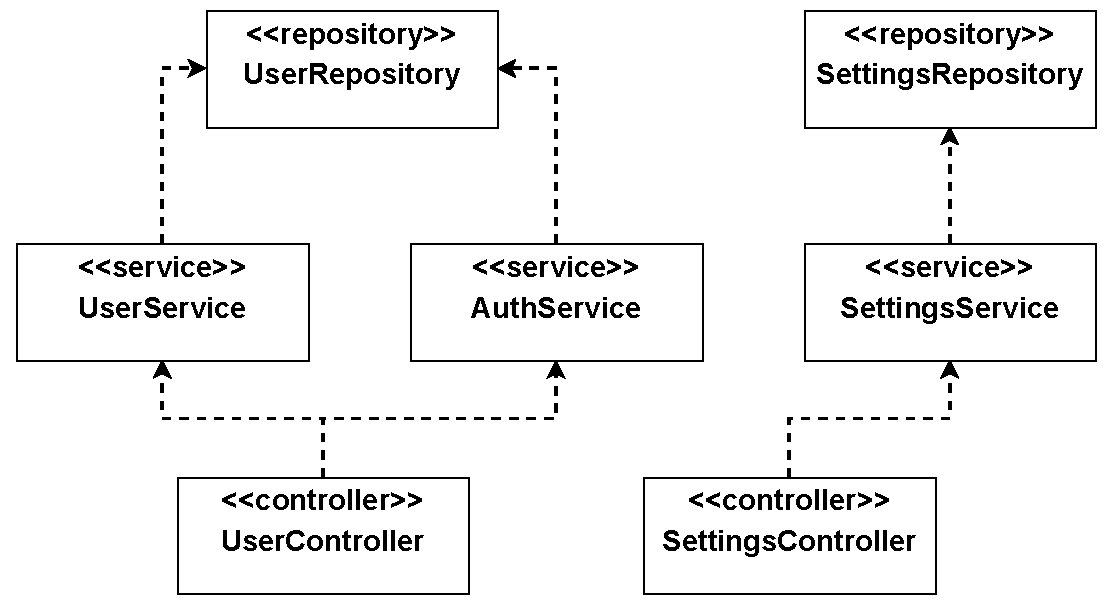
\includegraphics[width=1.0\linewidth]{flask.pdf}
    \caption{Diagram klas serwisu użykowników i ustawień}
    \label{rys:flask}
\end{figure}

Lista endpointów z opisem:
\begin{itemize}
    \item \texttt{/add\_user} -- dodawanie użytkownika;
    \item \texttt{/users} -- listowanie użytkowników;
    \item \texttt{/users\/[id]} -- operacje na konkretnym użytkowniku;
    \item \texttt{/login} -- zalogowanie użytkownika;
    \item \texttt{/logout} -- wylogowanie użytkownika;
    \item \texttt{/check\_session} -- zweryfikowanie sesji użytkownika;
    \item \texttt{/change\_password} -- zmiana hasła użytkownika;
    \item \texttt{/control/startSession} -- rozpoczęcie sesji sterowania robotem;
    \item \texttt{/settings} -- wylistowanie/zmiana ustawień;
    \item \texttt{/zerotier} -- połączenie do sieci \textit{ZeroTier};
    \item \texttt{/sftp} -- wylistowanie, zmiana ustawień transferu zdjęć przez SFTP;
    \item \texttt{/ip} -- informacja o adresach IP robota.
\end{itemize}

\section{Serwis sterujący silnikami robota}
\label{engine_service}
Główną funkcjonalnością tego programu jest przetwarzanie przychodzących komend sterowania silnikami robota i wykonywania ich.
Aplikacja napisana jest w języku Python i wystawia serwer \textit{Websockets}, wykorzystując nowoczesny framework do aplikacji internetowych \href{https://fastapi.tiangolo.com/}{\textit{FastAPI}}.
\textit{Websockets} to popularny protokół komunikacji używany w przeglądarkach internetowych.
Umożliwia ciągłą dwustronną komunikację w ramach jednego połączenia TCP.

Program serwuje też niewielkie REST API w celach zarządzania sesją.
Ten interfejs nie jest dostępny z zewnątrz, jedynie dla serwisu użytkowników \ref{main_backend}, który pośredniczy w inicjalizacji sesji tylko jeśli użytkownik jest już zautoryzowany.
Wtedy wydawany jest token sesji, który służy do autoryzacji do serwera Websocket.
Jeśli jakiś użytkownik ma już aktywną sesję sterowania silnikami, to nikt inny nie może takiej sesji zacząć do czasu aż sesja zostanie zakończona.
Proces ten przedstawiony jest na diagramie sekwencji \ref{rys:sequence}.

Serwer Websocket i REST są uruchamiane jako oddzielne procesy wymieniające się danymi przez kolejkę asynchroniczną.

\begin{figure}[H]
    \centering 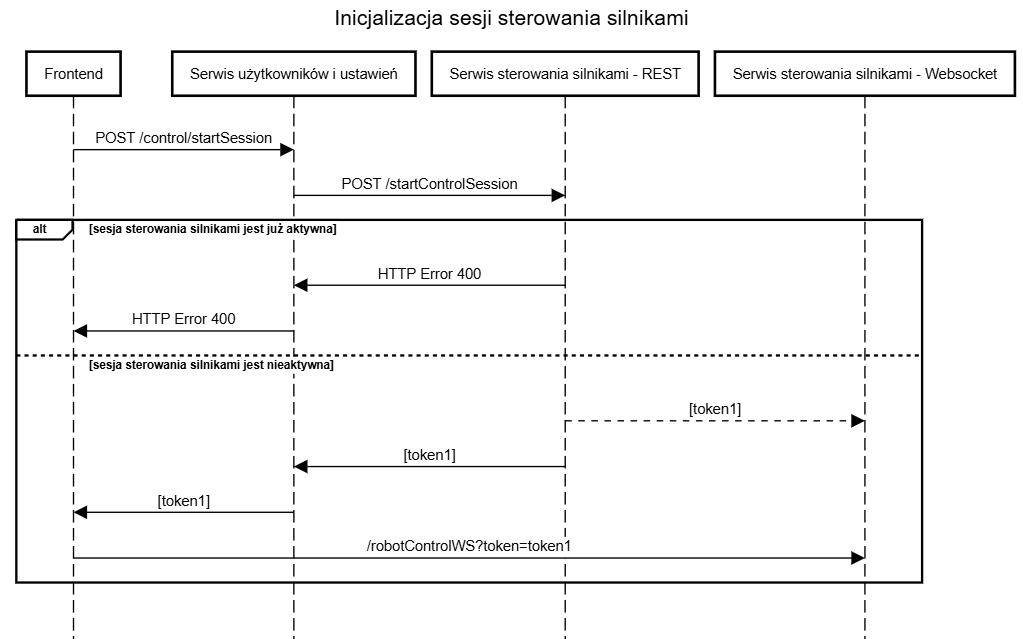
\includegraphics[width=1.0\linewidth]{robot_sequence.png}
    \caption{Diagram sekwencji inicjalizacji sesji sterowania silnikami}
    \label{rys:sequence}
\end{figure}

Wiadomości przesyłane przez Websocket mają popularny format JSON.
Przykładowa wiadomość:
\begin{verbatim}
{
    "type": "motorControl",
    "params": {
        "leftMotor": {
            "thrust": 50
        },
        "rightMotor": {
            "thrust": -25
        }
    }
}
\end{verbatim}
Wiadomość ta żąda włączenia 50\% mocy w lewym silniku i -25\% w prawym.
W przypadku braku nowych wiadomości od klienta w przeciągu pół sekundy, silniki zostają zatrzymane.
Komunikacja po interfejsie I\textsuperscript{2}C odbywa się za pomocą dostarczonej przez producenta sterownika silników \ref{motor_hat} biblioteki dla języka Python.

\section{Serwis kamery}
Funkcją tego programu jest strumieniowanie obrazu z kamery robota na żywo oraz regularne robienie zdjęć.
Jest on, podobnie jak serwis sterujący silnikami \ref{engine_service}, napisany w Pythonie i wykorzystuje framework \textit{FastAPI}.
Jako że do Raspberry Pi jest podpięta dedykowana kamera, to program może korzystać z dobrodziejstw dedykowanej biblioteki w języku Python - \href{https://picamera.readthedocs.io/en/release-1.13/#}{\textit{picamera}}.

Program strumieniuje obraz w formacie \textit{MotionJPEG}.
Jest to prosty format kompresji wideo typu intraframe -- każda klatka kompresowana jest oddzielnie w formacie JPEG.
Protokołem opakowującym jest HTTP.
Taki format strumieniowania wideo jest powszechnie wspierany przez przeglądarki internetowe.
Aplikacja wspiera rozsyłanie materiału do wielu klientów naraz.
Autoryzacja zapytań odbywa się przez ciasteczko sesji, które jest weryfikowane przez serwis użytkowników i ustawień \ref{main_backend}.

\section{Serwis archiwizacji zdjęć}
Rolą tego programu jest archiwizacja zrobionych zdjęć na zewnętrznym serwerze.
Aplikacja ta jest napisana w języku Python.
Pakuje wszystkie zdjęcia z podanego katalogu do formatu ZIP.
Następnie przesyła skompresowany plik na zdalny serwer za pomocą protokołu SFTP.
Namiary i dane autoryzacyjne są pobierane z lokalnej bazy danych -- z tej samej, z której korzysta serwis użytkowników i ustawień \ref{main_backend}.

We wdrożeniu program ten ma serwis uruchomieniowy \textit{systemd}.
Uruchamiany jest okresowo korzystając z systemu \textit{timer}-ów \textit{systemd}.

\section{Strona internetowa}
Oprogramowanie pełniące rolę interfejsu użytkownika to strona internetowa.
Pierwsza rzecz, którą widzi użytkownik po jej załadowaniu to ekran logowania, który jest pokazany na zrzucie ekranu \ref{rys:mob_login}.
\begin{figure}[!hb]
    \centering 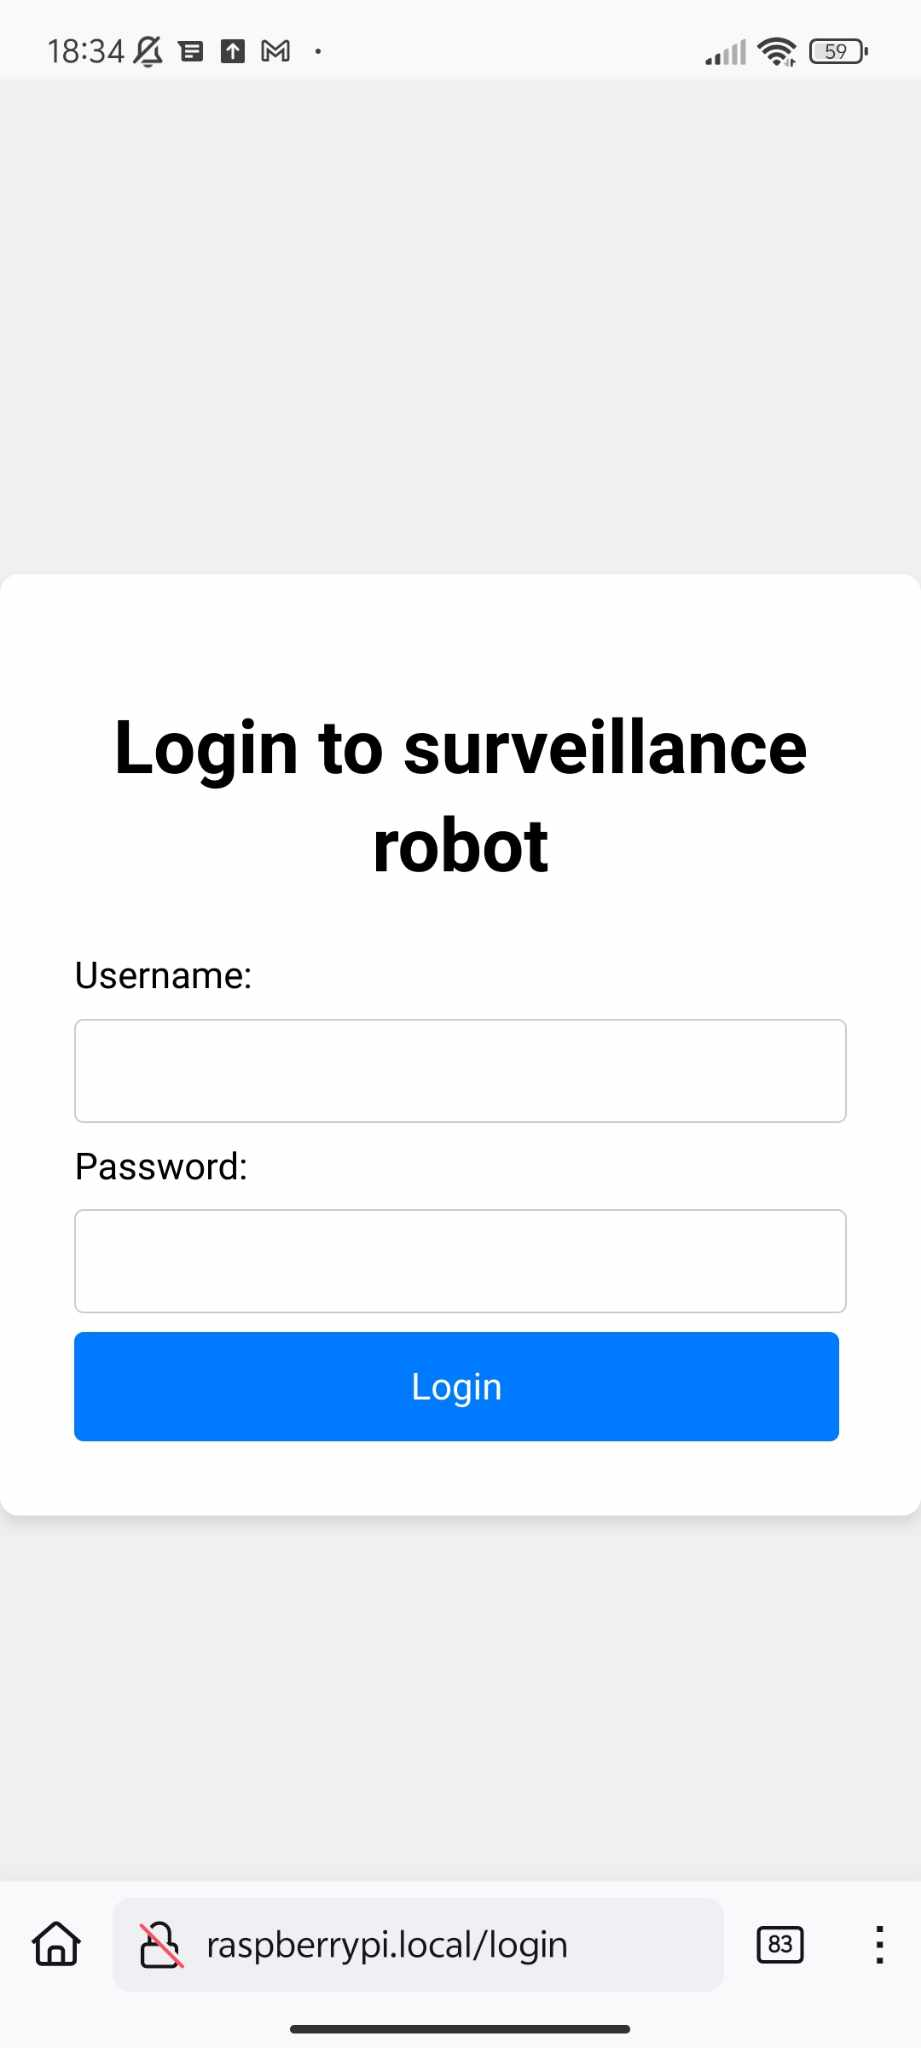
\includegraphics[width=0.3\linewidth]{mob_login.jpeg}
    \caption{Zrzut ekranu strony logowania na telefonie}
    \label{rys:mob_login}
\end{figure}
Po pomyślnym zalogowaniu ukazuje się strona główna.
Na niej jest wyświetlany podgląd z kamery robota.
Poniżej, automatycznie uruchamia się sesja i interfejs sterowania robotem.
Na górze są przyciski do przejścia do widoku ustawień lub wylogowania się.
Elementy te są zaprezentowane na zrzutach ekranu strony głównej na dużym ekranie: \ref{rys:front_desktop_main} i na ekranie telefonu: \ref{rys:mob_main}.
\begin{figure}[H]
    \centering 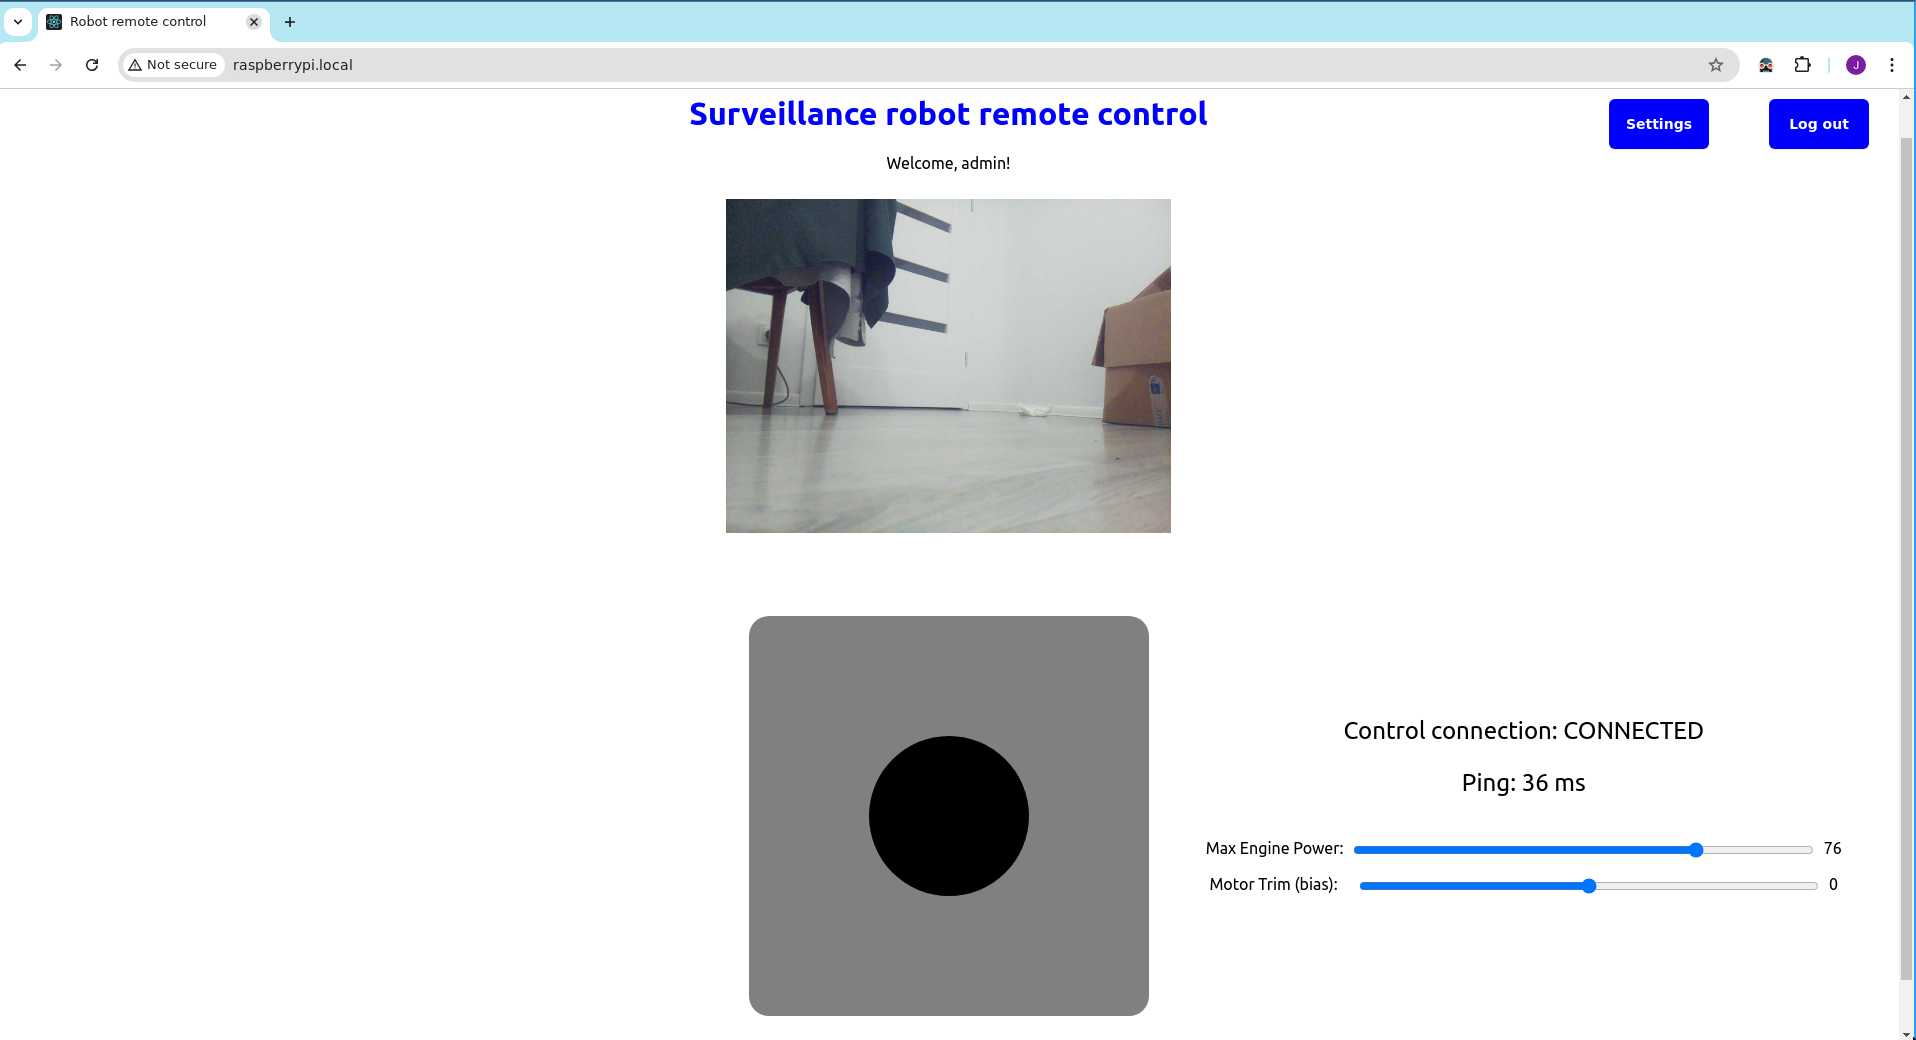
\includegraphics[width=1.0\linewidth]{front_desktop_main.png}
    \caption{Zrzut ekranu strony głównej na komputerze}
    \label{rys:front_desktop_main}
\end{figure}
\begin{figure}[H]
    \begin{subfigure}{.3\textwidth}
        \centering 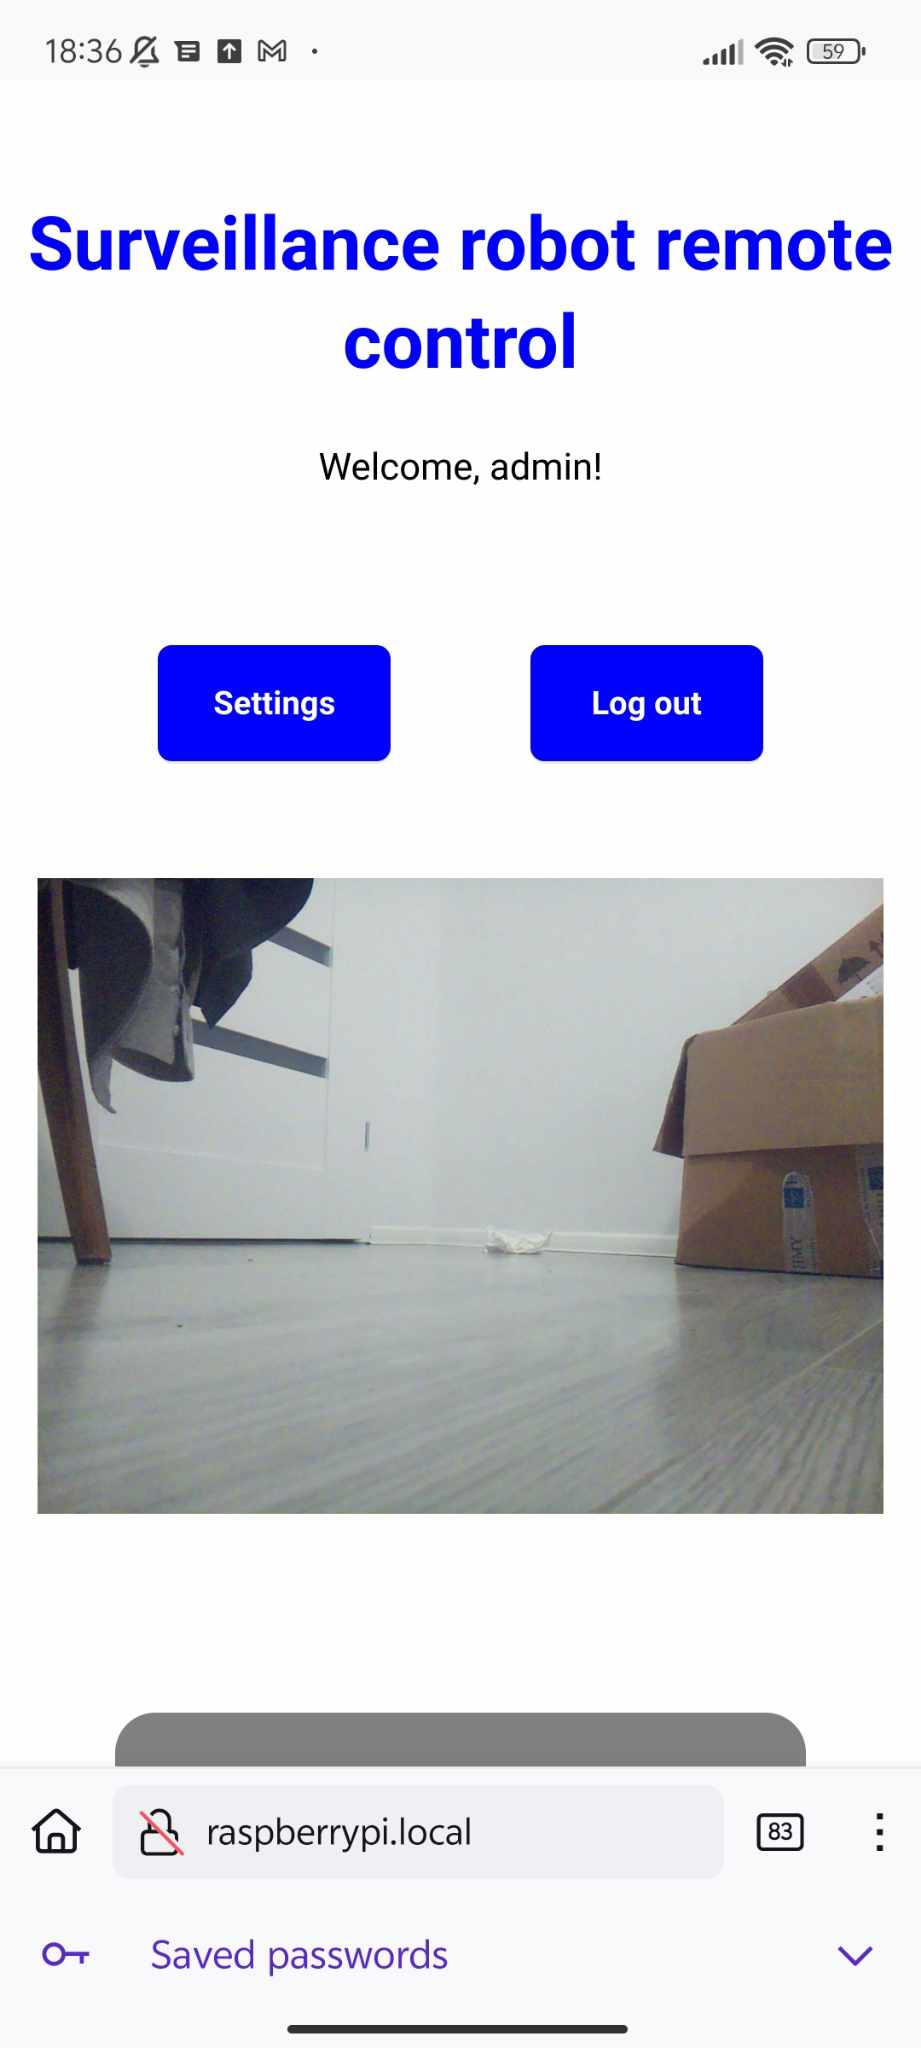
\includegraphics[width=0.8\linewidth]{mob_main.jpeg}
    \end{subfigure}
    \begin{subfigure}{.3\textwidth}
        \centering 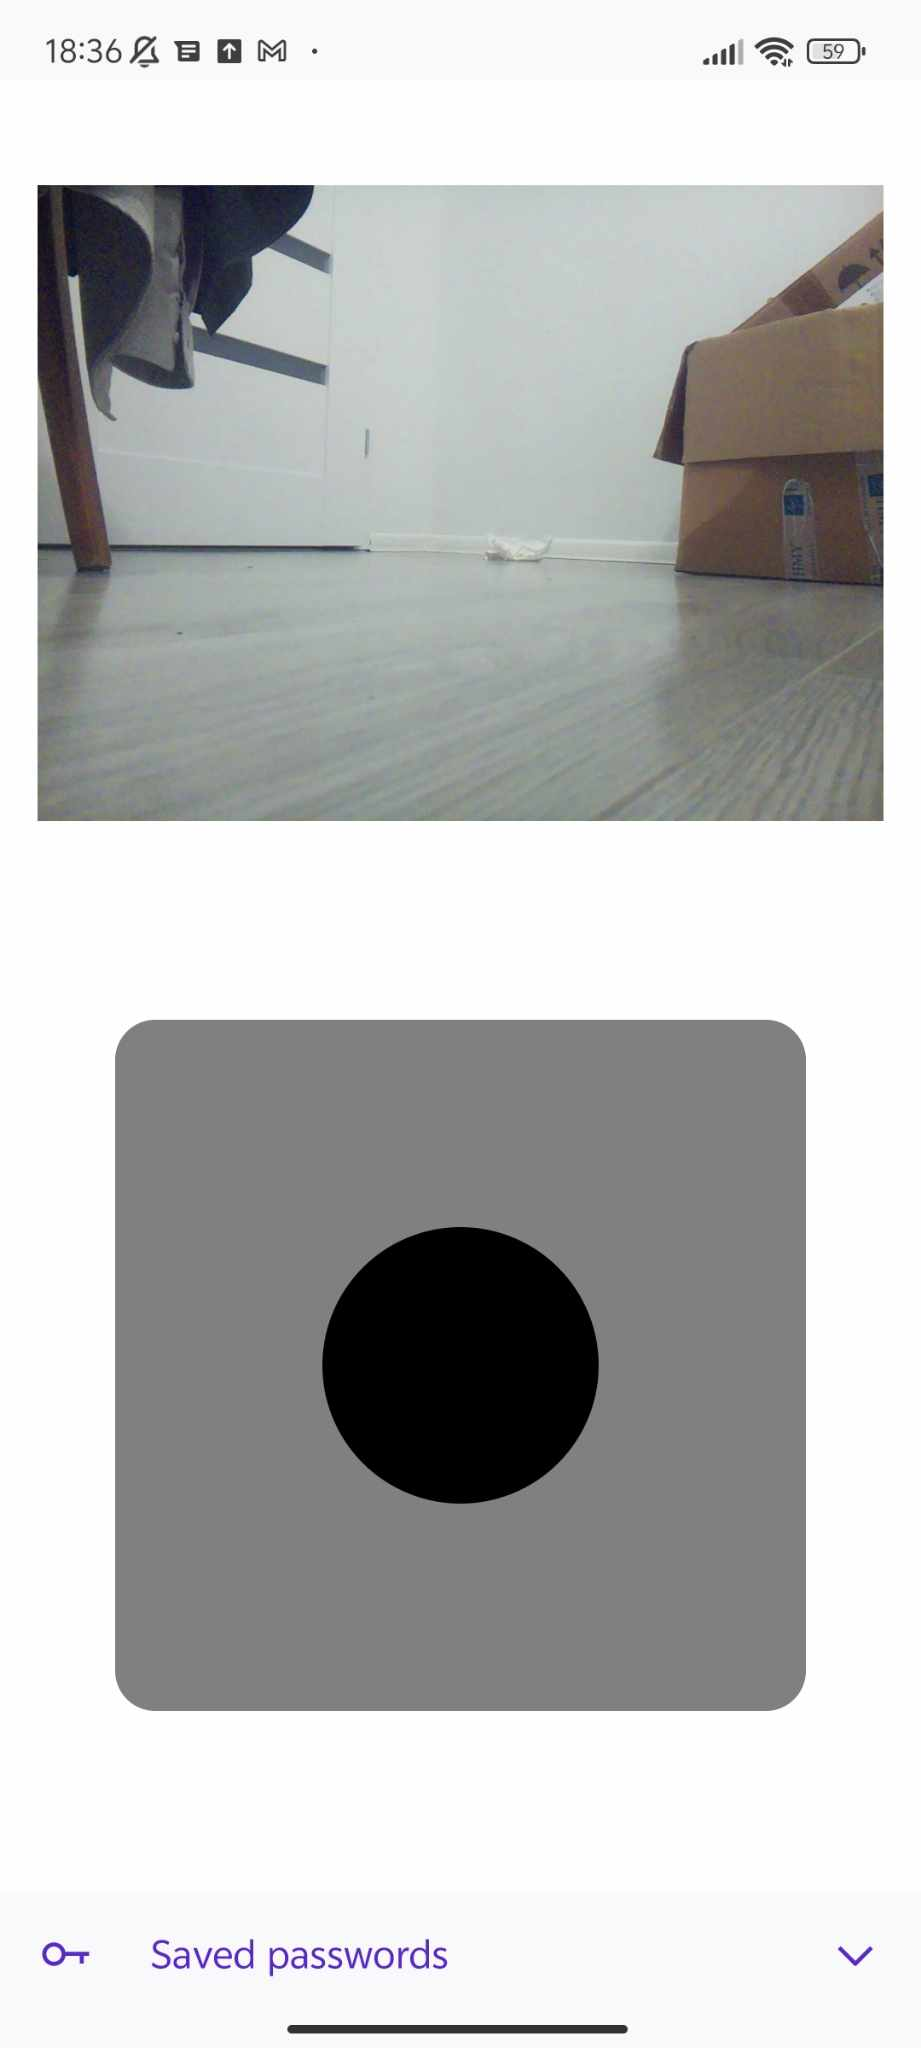
\includegraphics[width=0.8\linewidth]{mob_main3.jpeg}
    \end{subfigure}
    \begin{subfigure}{.3\textwidth}
      \centering 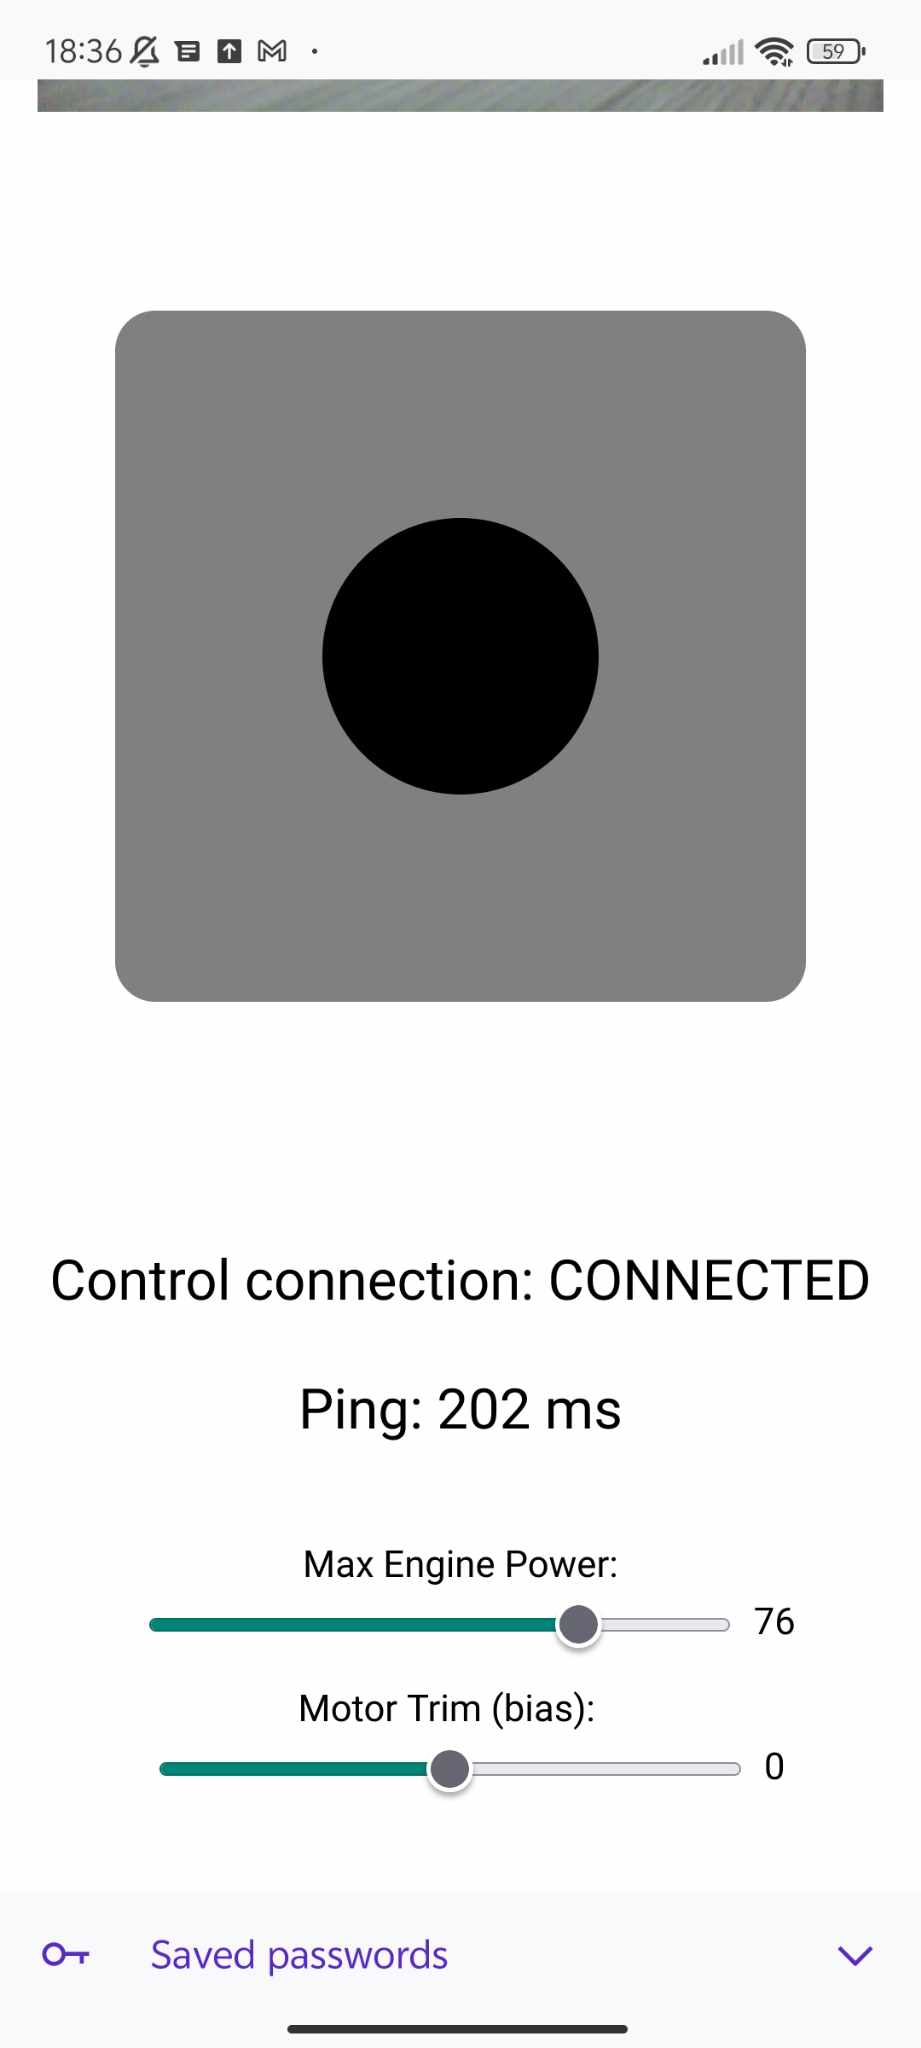
\includegraphics[width=0.8\linewidth]{mob_main2.jpeg}
    \end{subfigure}
    \caption{Zrzut ekranu strony głównej na telefonie}
    \label{rys:mob_main}
\end{figure}

Po kliknięciu odpowiedniego przycisku na stronie głównej otwiera się strona ustawień.
Jej wygląd jest ukazany na zrzutach ekranu w wersji na dużym ekranie: \ref{rys:front_desktop_set} i na ekranie telefonu: \ref{rys:mob_set}.
\begin{figure}[H]
    \centering 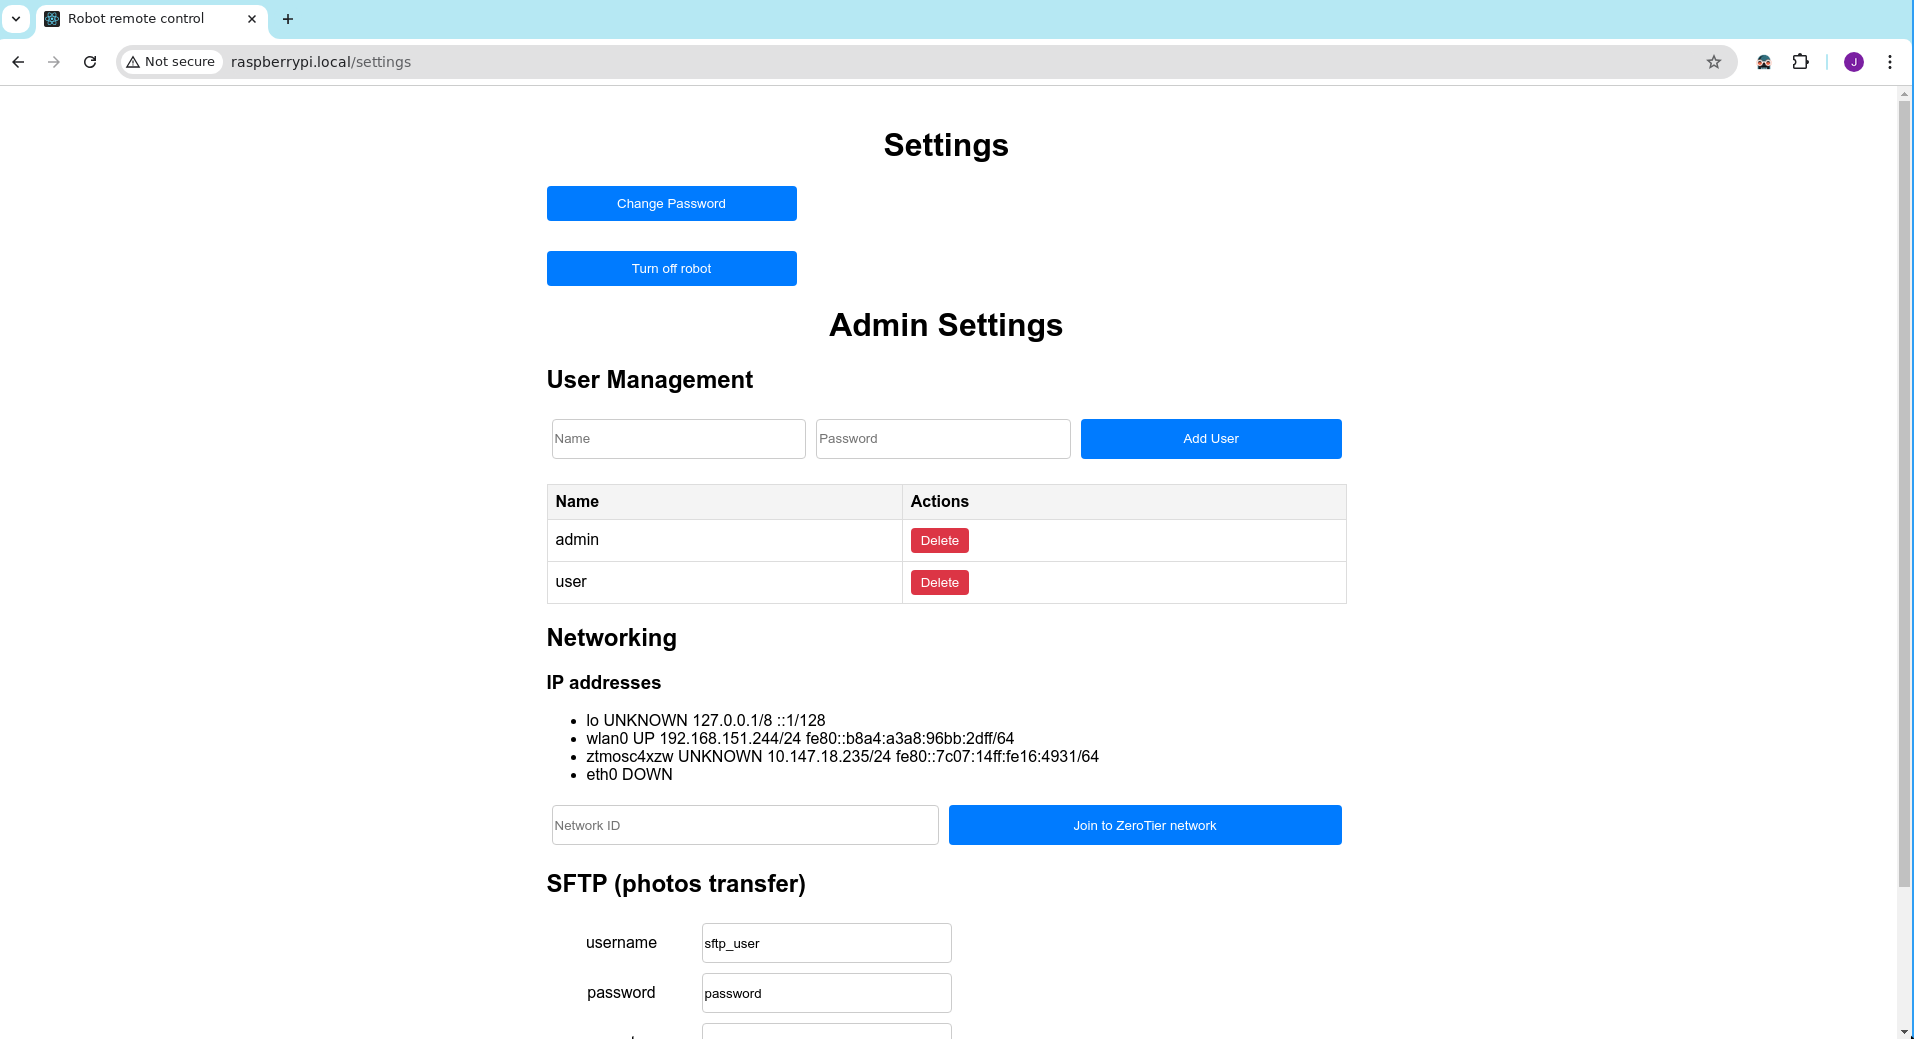
\includegraphics[width=1.0\linewidth]{front_desktop_set.png}
    \caption{Zrzut ekranu strony ustawień na komputerze}
    \label{rys:front_desktop_set}
\end{figure}
\begin{figure}[H]
    \centering 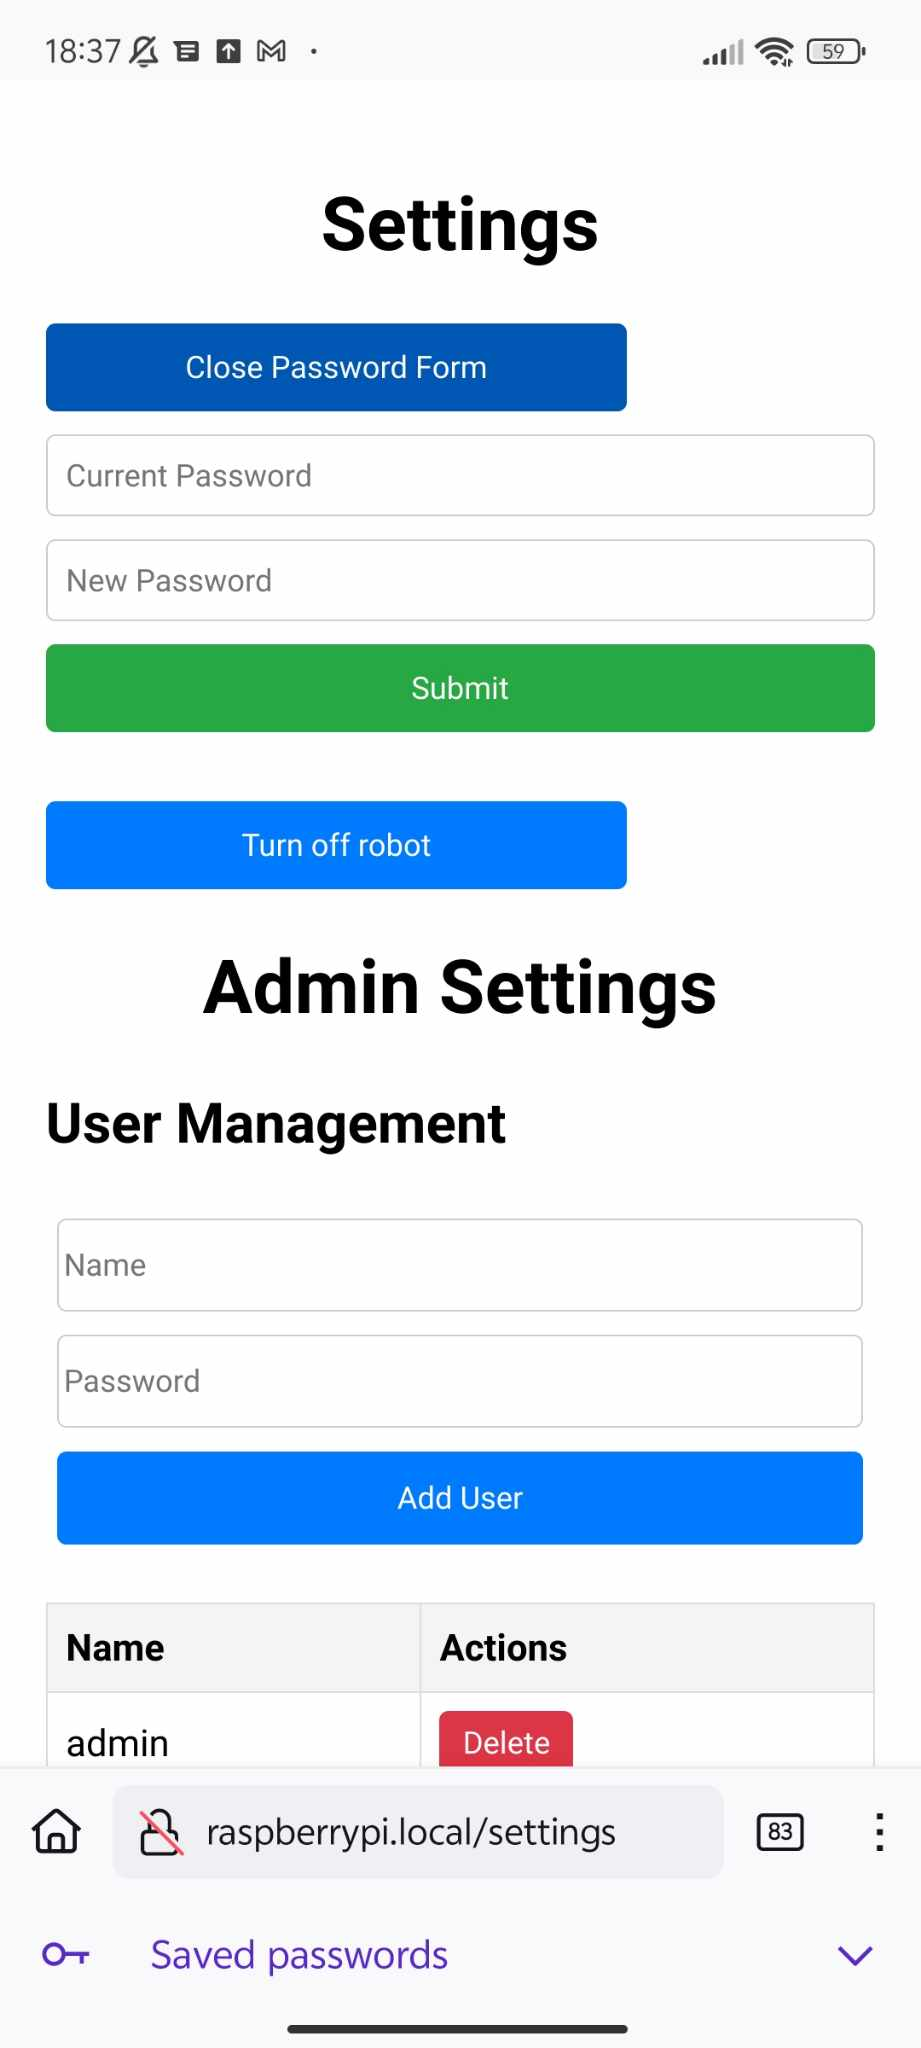
\includegraphics[width=.3\linewidth]{mob_set.jpeg}
    \caption{Zrzut ekranu strony ustawień na telefonie}
    \label{rys:mob_set}
\end{figure}
Z jej poziomu zwykły użytkownik może zmienić hasło do swojego konta bądź wyłączyć robota.

Administrator może:
\begin{itemize}
    \item dodać użytkownika,
    \item usunąć użytkownika,
    \item odczytać adresy IP na wszystkich interfejsach sieciowych robota,
    \item dodać robota do sieci VPN \textit{ZeroTier}
    \item odczytać i zmienić dane dostępowe serwera SFTP, gdzie archiwizowane są zdjęcia.
\end{itemize}

Jeśli chodzi o technologię wykonanie, to nie było tutaj możliwości szerokiego wyboru języków -- standardem są HTML i CSS do definicji wyglądu oraz JavaScript do zaprogramowania zachowania.
Został wykorzystany najpopularniejszy framework webowy dla Javascript-u -- \textit{React}.

\section{Moduł joysticka do sterowania ruchem robota}
Kod strony internetowej odczytuje pozycję joysticka i na jej podstawie oblicza wysterowanie silników.
Logika sterowania opiera się o algorytm, który przekłada pozycję joysticka na prędkość obrotową kół.
Do skręcania stosowana jest metoda sterowania różnicowego.
Im większy wychył joysticka do przodu/tyłu, tym większa prędkość obrotowa kół.
Im większy wychył joysticka w lewo/prawo, tym większa różnica prędkości obrotowej kół.
Kod odpowiedzialny za te obliczenia: \ref{lst:joystick_code}.
\begin{lstlisting}[language=C,
    caption={Kod obliczający moc silników na podstawie wychylenia joysticka},
    label={lst:joystick_code}]
function rescaleJoystickPos(posValue) {
    const pos = Math.abs(posValue) * 100
    if (pos <= JOYSTICK_DEADZONE) return 0
    else {
        return (pos - JOYSTICK_DEADZONE) / (100 - JOYSTICK_DEADZONE) * 100
    }
}
function handleJoystickMove(position) {
    const power = rescaleJoystickPos(position.y)
    const turn = rescaleJoystickPos(position.x)
    let outsideWheelSpeed = power
    let insideWheelSpeed = (100 - turn) * power / 100
    if (position.y < 0) {
        outsideWheelSpeed *= -1
        insideWheelSpeed *= -1
    }
    if (position.x > 0) {
        leftMotThrust.current = outsideWheelSpeed
        rightMotThrust.current = insideWheelSpeed
    } else {
        leftMotThrust.current = insideWheelSpeed
        rightMotThrust.current = outsideWheelSpeed
    }
}
\end{lstlisting}
Parametry wysterowania są wysyłane do serwera platformy nieustannie co stały interwał czasu.
